% $Id: introduction.tex 87303 2016-02-08 13:44:29Z lafferty $
%\begin{savequote}[8cm]
%\textlatin{Neque porro quisquam est qui dolorem ipsum quia dolor sit amet, consectetur, adipisci velit...}
%
%There is no one who loves pain itself, who seeks after it and wants to have it, simply because it is pain...
%  \qauthor{--- Cicero's \textit{de Finibus Bonorum et Malorum}}
%\end{savequote}

\chapter{\label{ch:2-background}\CP violation and measurements of CKM angle \Pgamma} 

\minitoc

\section{The Standard Model}

The Standard Model (SM) of particle physics describes all known fundamental particles and their interactions. Its predictions have been rigorously tested over several decades and have found to be consistent with our observations to remarkable levels of precision. Although the SM has proven to be extremely accurate it has several limitations, for example the model does not incorporate gravitational interactions, provide a dark matter candidate, or explain the huge asymmetry observed between matter and antimatter. These problems suggest that the SM is an incomplete theory, hence experimental particle physics is driven by the search for direct or indirect signs of New Physics (NP).

The SM contains twelve spin-1/2 fermions in three generations, which are grouped in quarks and leptons, listed in Table \ref{SMfermions}. These fermions interact via the electromagnetic, weak and strong forces, which are mediated by gauge bosons listed in Table \ref{SMbosons}. The Brout-Englert-Higgs boson ($BEH$) is the only elementary scalar particle, and it couples to all particles with mass. The Higgs mechanism explains why weak gauge bosons have mass, while the photon is massless. All these elementary particles have corresponding antiparticles.

Quarks do not exist as free particles, but always exist in bound states with other quarks, referred to as hadrons. There are two different types of hadrons, known as mesons and baryons. Mesons are two-particle bound states composed of a quark and an antiquark, and baryons are three-particle bound states composed of three quarks. Examples of meson include \B mesons, containing a \bquark or \bquarkbar quark, \eg \Bm, \Bp, \Bz, and \D mesons, containing a \cquark or \cquarkbar quark, \eg \Dm, \Dp, \Dz. Examples of baryons include protons, containing \uquark\uquark\dquark quark composition, and \Lz baryons, containing \uquark\dquark\squark quark composition.

\begin{table}
\centering
\begin{tabular}{c|cc|cc}
& \multicolumn{2}{p{6cm}}{\hspace{2.2cm} Quarks} & \multicolumn{2}{p{6cm}}{\hspace{2.2cm} Leptons} \\
& Flavour & Charge & Flavour & Charge \\
\hline \hline
First generation & up (\uquark) & $+2/3$ & electron (e) & $-1$ \\
 & down (\dquark) & $-1/3$ & electron neutrino (\neue) & $0$ \\
\hline
Second generation & charm (\cquark) & $+2/3$ & muon (\muon) & $-1$ \\
 & strange (\squark) & $-1/3$ & muon neutrino (\neum) & $0$ \\
\hline
Third generation & top (\tquark) & $+2/3$ & tau (\tauon) & $-1$ \\
 & bottom (\bquark) & $-1/3$ & tau neutrino (\neut) & $0$ \\
\end{tabular}
\caption{Quarks and leptons in the Standard Model.}
\label{SMfermions}
\end{table}

\begin{table}
\centering
\begin{tabular}{c|cc}
Gauge boson & Force & Charge \\
\hline
photon (\g) & Electromagnetic & $0$ \\
\Z & Weak & $0$ \\
\Wpm & Weak & $\pm 1$ \\
gluon ($g$) & Strong & $0$ \\
\hline
BEH (scalar) & - & $0$
\end{tabular}
\caption{Gauge bosons in the Standard Model. The Brout-Englert-Higgs boson ($BEH$) is not a Gauge boson, but a neutral scalar boson, which couples to all particles with mass.}
\label{SMbosons}
\end{table}

\section{\CP violation}

One of the key problems with the SM is that is does not explain why our universe consits almost entirely of matter, with hardly any antimatter present. This asymmetry is commonly quantified by the baryon-antibaryon asymmetry, $\frac{n_{B} - n_{\bar{B}}}{n_{\g}} \approx \frac{n_{B}}{n_{\g}}$, where $n_{B}$, $n_{\bar{B}}$ and $n_{\g}$ are the baryon, anti-baryon and photon number densities respectively. Astrophysical observations have measured the baryon-antibaryon asymmetry to be of the order of $10^{-10}$~\cite{astrophysicalasy}. The requirements for this asymmetry to be generated from a symmetrical initial state, known as baryogenisis, were first proposed by Andrei Sakharov in 1967~\cite{sakharov}. These three Sakharov conditions are: baryon number violation, the violation of charge ($C$) symmetry and charge-parity (\CP) symmetry, and departure from thermal equilibrium. These components are required in all baryogenisis models. The definitions of the $C$ and $P$ symmetries are given by their operators:
\begin{itemize}
\item The charge conjugation operator, $\hat{C}$, converts particles into their antiparticles.
\item The parity operator, $\hat{P}$, reverses the spacial axis so all vectors change sign.
\end{itemize}
\CP symmetry is violated if the system changes under the combined $\hat{C}\hat{P}$ transformation.

The SM satisfies all necessary conditions for baryogenisis, however the amount of asymmetry that can be generated from \CP violation in the SM is many orders of magnitude smaller than the asymmetry observed from astrophysical observations~\cite{SMasy}. New Physics models that introduce new sources of \CP violation{\color{red}{[ref]}}, such as supersymmetric models, can be developed by theorists and searched for at the LHC and other experiments. However, it is also necessary to make precise measurements of \CP violation in the SM to improve our understanding of matter-antimatter asymmetry and search for indirect signs of New Physics.

\CP violation (CPV) is probed using many different processes. The different types of \CP violation in the SM can be split into three categories:
\begin{itemize}
\item \textbf{Direct CPV in decay}: this is when the rate of decay of a particle is not equal to the rate of the decay of the corresonding antiparticle \eg
\begin{equation*}
\Gamma\left(\decay{\Bm}{\D\Km}\right) \neq \Gamma\left(\decay{\Bp}{\D\Kp}\right)
\end{equation*}
\item \textbf{Indirect CPV in mixing}: Neutral mesons can oscillate between their particle and antiparticle states, $\Bz \leftrightarrow \Bzb$, as shown in Figure \ref{mixing}. Indeirect \CP violation occurs when \decay{\Bz}{\Bzb} and \decay{\Bzb}{\Bz} proceed at different rates. 
\begin{figure}[h]
\centering
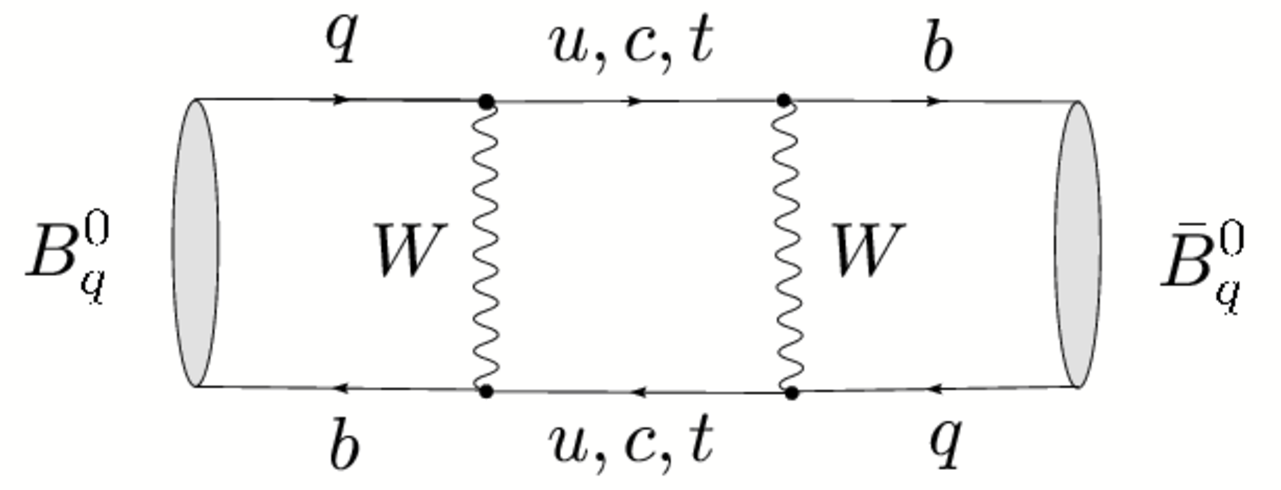
\includegraphics[width=0.5\linewidth]{figures/theory/mixing.pdf}
\caption{Feynman diagram of mixing between \Bz and \Bzb.}
\label{mixing}
\end{figure}
\item \textbf{CPV from the interference of mixing and decay}: A \Dz meson can decay to a \Kp\pim final state via a doubly Cabibbo suppressed decay. However, this process can also proceed via \decay{\Dz}{\Dzb} mixing, where the \Dzb decays to \Kp\pim, via a Cabibbo favoured decay. These two decay paths to the same final states interfere with each other, which cna result in another form of \CP violation.
\end{itemize} 

\section{The CKM matrix}

Quarks in the Standard Model can interact via the strong, weak or electromagnetic interactions. The weak interaction couples to a rotation of the flavour eigenstates.
Therefore, the eigenstates that take part in the weak interaction (weak eigenstates) are different to the flavour eigenstates that hadronise to produce the observable meson states. The Cabibbo-Kobayashi-Maskawa (CKM) matrix, $V_{CKM}$, given in \eqn \ref{CKMmatrix}, describes the relationship between the weak eigenstates ($d'$, $s'$, $b'$) and flavour eigenstates (\dquark, \squark, \bquark) of the quarks. 
\begin{equation}
\left(
\begin{array}{c} d' \\ s' \\ b'  \end{array} \right) =
\begin{pmatrix} V_{ud} & V_{us} & V_{ub} \\ V_{cd} & V_{cs} & V_{cb} \\ V_{td} & V_{ts} & V_{tb} \end{pmatrix} \left( 
\begin{array}{c} d \\ s \\ b \end{array} \right) =
V_{CKM} \left( \begin{array}{c} d \\ s \\ b \end{array} \right)
\label{CKMmatrix}
\end{equation}
The elements of this matrix, $V_{ij}$, define the coupling of a $j \to i$ quark transition. Similarly $V_{ij}^*$ define the coupling of a $\bar{j} \to \bar{i}$ antiquark transition. By definition the CKM matrix, $V_{CKM}$, is unitary, i.e. $V_{CKM}V_{CKM}^* = \mathds{1}$, assuming there are only three generations of quarks. The CKM matrix is a complex, $3 \times 3$ matrix, which yields 18 parameters. The unitarity requirement, coresponding to nine complex equations, reduces the number of free parameters, and five strong phases can be absorbed into the quark fields as they are not physically observable. This leave four independent free parameters to describe the CKM matrix: three amplitudes and one phase. This free phase parameter is the source of \CP violation in the SM. 

A standard representation of the CKM matrix uses 3 angles, $\theta_{12}$, $\theta_{23}$ and $\theta_{13}$, and one \CP violating phase, $\delta$, as shown in Equation \ref{standard}. Couplings between the quark generation $i$ and $j$ vanish if $\theta_{ij} = 0$, and $s_{ij}$ and $c_{ij}$ represent $\sin\theta_{ij}$ and $\cos\theta_{ij}$.
\begin{equation}
V_{CKM} = \begin{pmatrix} 1 & 0 & 0 \\ 
0 & c_{23} & s_{23} \\ 
0 & -s_{23} & c_{23} \end{pmatrix}
\begin{pmatrix} c_{13} & 0 & s_{13}e^{-i\delta_{13}} \\ 
0 & 1 & 0 \\ 
-s_{13}e^{i\delta_{13}} & 0 & c_{13} \end{pmatrix}
\begin{pmatrix} c_{12} & s_{12} & 0 \\ 
-s_{12} & c_{12} & 0 \\ 
0 & 0 & 1 \end{pmatrix}
\label{standard}
\end{equation}

If the CKM matrix was equivalent to the identity matrix there would be no cross-generation weak interaction of the quarks \eg\ a \uquark quark transition mediated by a W boson could only result in a \dquark, not a \squark or \bquark quark. From empirical determination, the magnitude of the elements in the CKM matrix are~\cite{PDG2016}:
\begin{equation}
| V_{CKM} | = \begin{pmatrix} 0.97434^{+0.00011}_{0.00012} & 0.22506 \pm 0.00050 & 0.00357 \pm 0.00015 \\ 0.22492 \pm 0.00050 & 0.97351 \pm 0.00013 & 0.0411 \pm 0.0013 \\ 0.00875^{+0.00032}_{-0.00033} & 0.0403 \pm 0.0013 & 0.99915 \pm 0.00005 \end{pmatrix}
\end{equation}
It can be seen that quark transitions within the same generation is highly favoured, these are known as Cabibbo-favoured decays. Also, quark transitions across one generation are suppressed, and are even more suppressed across two generations. These are known as Cabibbo-suppressed transitions. 

This structure in the CKM matrix is illustrated by the Wolfenstein parameterisation, given in Eq.~\ref{wolf}, which uses parameters, $A$, $\lambda$, $\rho$ and $\eta$. 
\begin{equation}
V_{CKM} = \begin{pmatrix} 1 - \lambda^2/2 & \lambda & A\lambda^3(\rho - i\eta) \\ 
-\lambda & 1 - \lambda^2/2 & A\lambda^2 \\ 
A\lambda^3(1 - \rho - i\eta) & -A\lambda^2 & 1 \end{pmatrix}
\label{wolf}
\end{equation} 
This is an approximation of the standard parameterisation given in Eq.~\ref{standard}, expanded in powers of the small parameter $\lambda = \sin\theta_{12} = 0.22$. The other parameters are deinfed by, $A\lambda^2 = s_{23}$ and $A\lambda^3(\rho - i\eta) = s_{13}e^{-i\delta}$. The \CP violation can be determined by measuring $\rho - i\eta$.

\section{The CKM unitarity triangle}

Verifying the unitarity of the CKM matrix is of the utmost importance since non-unitarity is a clear sign of physics Beyond the Standard Model~\cite{CKMtriangle}. The unitarity of the CKM matrix leads to nine unitarity conditions, for example $\Vud\Vubs + \Vcd\Vcbs + \Vtd\Vtbs = 0$, which is the most easily applicable to \B physics. These relations can be represented as a triangle in the complex plane, as shown in Figure \ref{triangle}. The triangle representing the condition $\Vud\Vubs + \Vcd\Vcbs + \Vtd\Vtbs = 0$ is often chosen as all the quantities are experimentally measurable and are of reasonable relative size; it has angles $\alpha$, $\beta$ and \Pgamma, and an area proportional to the amount of \CP violation in the quark sector of the Standard Model~\cite{CKMtriangle}. 
\begin{figure}
\centering
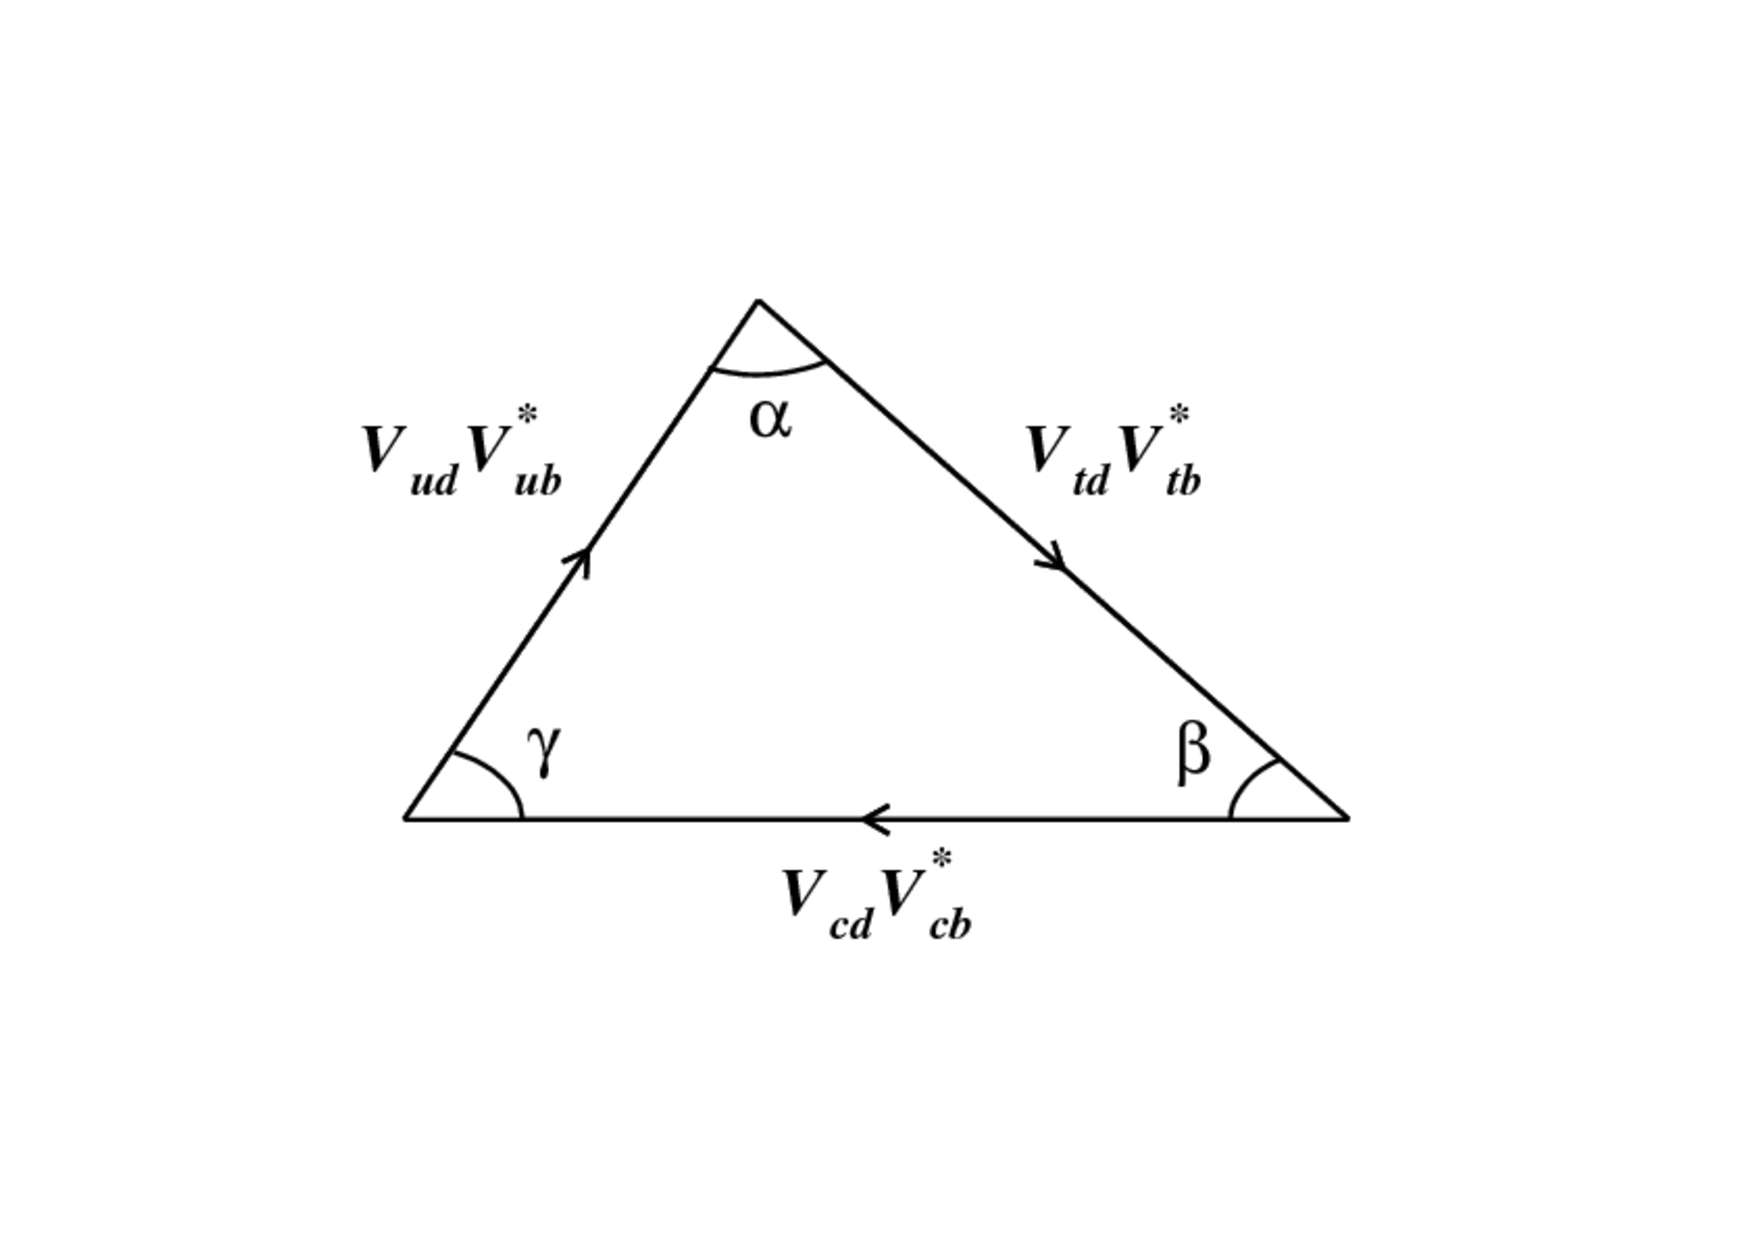
\includegraphics[width=0.4\linewidth]{figures/theory/triangle.pdf}
\caption{CKM triangle}
\label{triangle}
\end{figure}

The values of $\alpha$, $\beta$ and \Pgamma can be accessed by looking at various \B meson decays. Overconstraining this unitarity triangle, will allows verification as to whether or not the triangle closes, i.e. whether it truely is a triangle. Obtaining inconsistent results when overconstraining the unitarity triangle would suggest that the CKM is not unitary, which is incompatible with the Standard Model. 

The CKM angle $\Pgamma \equiv \arg\left(-\frac{\Vud{\Vub}^*}{\Vcd{\Vcb}^*}\right)$ in the angle with the largest uncertainty in the CKM unitarity triangle. This angle is measured using the \lhcb detector from the rates of decays of a range of different decays that can be generalised as, charged and neutral \B decays to a \D meson (reconstructed in one of a variety of final states) and a kaon. These are known as direct measurements. In order to obtain the most precise direct measurement of \Pgamma, the individual measurements from each of these \Pgamma-sensitive decays are combined to produce a single value with a lower uncertainty. The latest published \lhcb combination is $\Pgamma = \left(72.2^{+6.8}_{-7.3}\right)^{\circ}$~\cite{LHCb-PAPER-2016-032}. This is the most precise determination of \Pgamma from direct measurements from a single experiment; other experiments are consistent, but less precise. These direct measurements of \Pgamma involve only tree level process, making them theoretically clean. New particles that are not predicted in the Standard Model can only enter at higher order, and are therefore highly suppressed. As \Pgamma can be determined at tree-level, direct measurements are dominated by Standard Model contributions.

A global fit to the CKM triangle from CKMfitter~\cite{CKMFitter}, shown in \fig\ref{globalfit}, uses the current best measurements of various quantities, such as $\beta$, $\Delta m_d$ and $\Delta m_s$, as inputs, where $\Delta m_d$ and $\Delta m_s$ are the mass difference between the mass eigenstates of \Bz-\Bzb and \Bs-\Bsb respectively. When performing this fit any information on \Pgamma from direct measurements is ignored. Assuming the Standard Model, i.e. unitarity of CKM matrix, \Pgamma is extracted. The measurements for these inputs used include loop processes. The presence of the loop in the Feunman diagram allows additional Beyond the Standard Model diagrams, where new particles appear in the loop contributing to the amplitude at the same order. Therefore, these loop processes are sensitive to New Physics. This method obtains a \Pgamma measurement of $(66.9^{+0.9}_{-3.4})^{\circ}$, where this determination of \Pgamma excludes all direct measurements and assumes the Standard Model. The leading uncertainties on the indirect measurement are from lattice QCD; these uncertainties are expected to decrease as lattice QCD calculations become more accurate. 
\begin{figure}[!ht]
\centering
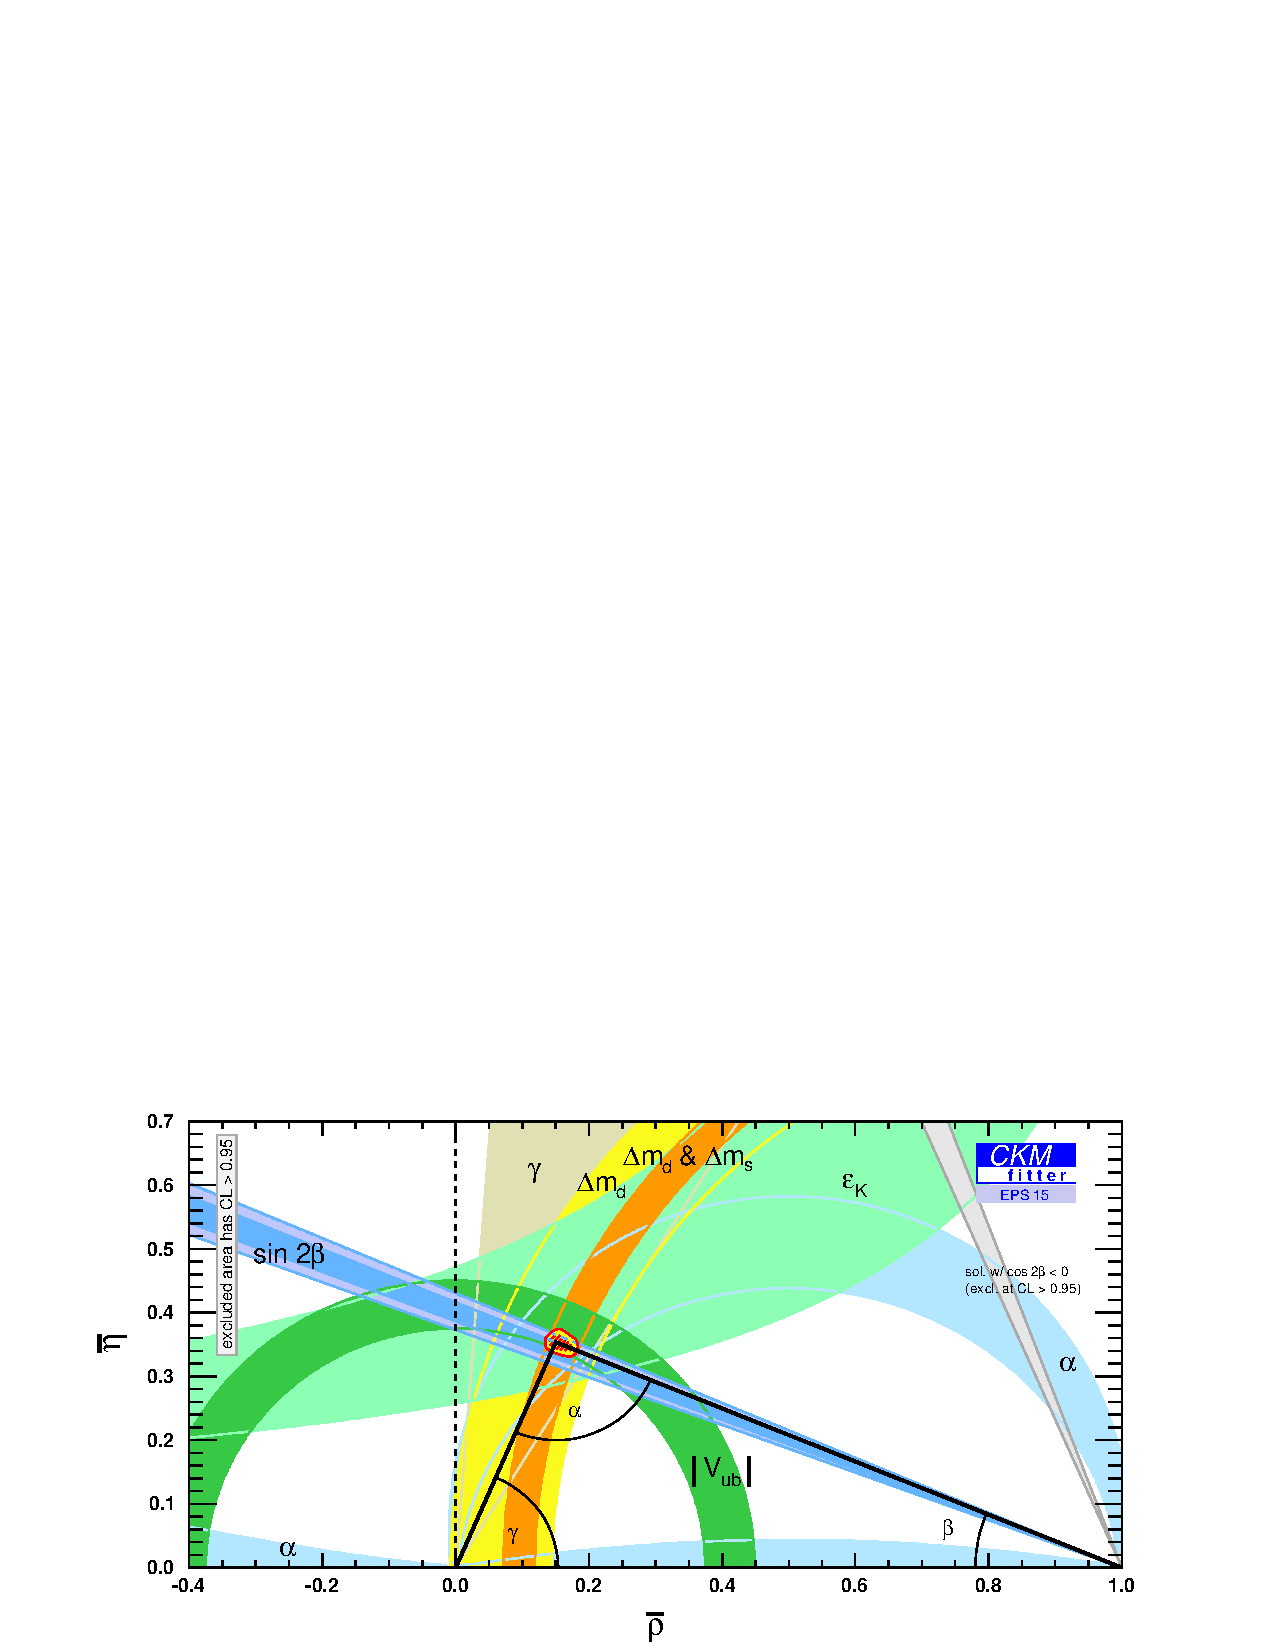
\includegraphics[trim = 0mm 0mm 0mm 180mm,clip,width=0.9\linewidth]{figures/theory/rhoeta_small_global.pdf}
\caption{Diagram showing the current state of measurements of the unitarity triangle. The black line shows the fit obtained by CKM fitter}
\label{globalfit}
\end{figure}

The direct and indirect measurements of \Pgamma are currently consistent with each other, however, the result of \Pgamma from direct measurements has a relatively large uncertainty and higher central value. Therefore, improving the precision of the direct measurement of \Pgamma is necessary to verify whether or not the direct and indirect measurements are consistent, thereby testing the consistency of the Standard Model. Improvements in the precision can be achieved through a combination of measurements of various \B decays that are sensitive to \Pgamma.

\section{Tree-level determination of \Pgamma using \decay{\Bpm}{\D K^{(*)\pm}} decays}
\label{sec:theory:gamma}

Direct measurements of \Pgamma can be made by exploiting the interference between \decay{\bquark}{\cquark\uquarkbar\squark} and \decay{\bquark}{\uquark\cquarkbar\squark} transitions. These transitions are present at tree-level in $\Bpm \to \D\kaon^{(*)\pm}$ decays, represented by the Feynman diagrams shown in \fig\ref{fig:B2DKstarmdiagram}, showing \decay{\Bm}{\Dz\Kstarm} (left) and \decay{\Bm}{\Dzb\Kstarm} (right). The branching
fraction is of similar order to \decay{\Bm}{\Dzb\Km} which has been extensively analysed at~\cite{LHCb-PAPER-2016-003,LHCb-PAPER-2014-041,LHCb-PAPER-2015-014}.
\begin{figure}[!h]
\centering
\resizebox{0.48\linewidth}{!}{
	\begin{tikzpicture}[scale=0.98]
        % MAP OUT VERTICES (I have 8 of them)
        \coordinate (a) at (0,2); %b quark start
        \coordinate (b) at (0,1); %ubar quark start
        \coordinate (c) at (5,1); %ubar quark end
        \coordinate (d) at (5,2); %c quark end
        \coordinate (e) at (2,2); %start the W+
        \coordinate (f) at (5,2.67); %s quark
        \coordinate (g) at (5,3.33); %ubar quark
        \coordinate (h) at (4.0,3); %W end
        % DRAW LINES
        \draw[antiparticle] (b)  -- (c); %ubar quark
        \draw[particle] (a)  -- (e); %bbar quark
        \draw[particle] (e)  -- (d); %ubar quark 
        \draw[photon] (e) -- (h); %W+
        \draw[antiparticle] (h)  to (g); %W to ubar quark
        \draw[particle] (h)  to (f); %W to s quark 
        %DRAW LABELS
        \node at ($(a)$) [label={[label distance=-4mm] b},left] {};
        \node at ($(b)$) [label={[label distance=-4mm] $\bar{\rm u}$},left] {};
        \node at ($(c)$) [label={[label distance=-4mm] $\bar{\rm u}$},right]{};
        \node at ($(d)$) [label={[label distance=-4mm] c},right] {};
        \node at ($(f)$) [label={[label distance=-4mm] s},right] {};
        \node at ($(g)$) [label={[label distance=-4mm] $\bar{\rm u}$},right]{};
        \node at ($(e)$) [label={[xshift=25pt,yshift=10pt] $W^-$},above] {};

        %ADD BRACES
        \draw
        [black,decorate,decoration={brace,amplitude=5pt},xshift=-20pt,yshift=0pt]
          (0,0.8)  -- (0,2.2) node [black,midway,left=0pt,xshift=-5pt]{$\Bm$};
        \draw
        [black,decorate,decoration={brace,amplitude=5pt},xshift=20pt,yshift=0pt]
          (5,3.53) -- (5,2.47) node [black,midway,right=0pt,xshift=5pt]{$\Kstarm$};
         \draw 	[black,decorate,decoration={brace,amplitude=5pt},xshift=20pt,yshift=0pt]
          (5,2.2)  -- (5,0.8) node [black,midway,right=0pt,xshift=5pt] {$\Dz$};
            \end{tikzpicture}
        }
\resizebox{0.47\linewidth}{!}{
\begin{tikzpicture}[scale=0.98]
        % MAP OUT VERTICES (I have 8 of them)
        \coordinate (a) at (0,3); %b quark start
        \coordinate (b) at (0,1); %ubar quark start
        \coordinate (c) at (5,1); %ubar quark end
        \coordinate (d) at (5,3); %u quark end
        \coordinate (e) at (2,3); %start the W+
        \coordinate (f) at (5,1.67); %s quark
        \coordinate (g) at (5,2.33); %cbar quark
        \coordinate (h) at (4.0,2); %W end
        % DRAW LINES
        \draw[antiparticle] (b)  -- (c); %ubar quark
        \draw[particle] (a)  -- (e); %b quark
        \draw[particle] (e)  -- (d); %u quark 
        \draw[photon] (e) -- (h); %W+
        \draw[antiparticle] (h)  to (g); %W to cbar quark
        \draw[particle] (h)  to (f); %W to s quark 
        %DRAW LABELS
        \node at ($(a)$) [label={[label distance=-4mm] b},left] {};
        \node at ($(b)$) [label={[label distance=-4mm] $\bar{\rm u}$},left] {};
        \node at ($(c)$) [label={[label distance=-4mm] $\bar{\rm u}$},right]{};
        \node at ($(d)$) [label={[label distance=-4mm] u},right] {};
        \node at ($(f)$) [label={[label distance=-4mm] s},right] {};
        \node at ($(g)$) [label={[label distance=-4mm] $\bar{\rm c}$},right]{};
        \node at ($(e)$) [label={[xshift=25pt,yshift=-40pt] $W^-$},above] {};

        %ADD BRACES
        \draw 	[black,decorate,decoration={brace,amplitude=5pt},xshift=-20pt,yshift=0pt]
        (0,0.8)  -- (0,3.2) node [black,midway,left=0pt,xshift=-5pt] {$\Bm$};
        \draw [black,decorate,decoration={brace,amplitude=5pt},xshift=20pt,yshift=0pt]
        (5,1.85)  -- (5,0.8) node [black,midway,right=0pt,xshift=5pt] {$\Kstarm$};
         \draw [black,decorate,decoration={brace,amplitude=5pt},xshift=20pt,yshift=0pt]
        (5,3.2)  -- (5,2.15) node [black,midway,right=0pt,xshift=5pt] {$\bar{\rm \Dz}$};
        \end{tikzpicture}
    }
    \caption{Leading order Feynman diagrams for \decay{\Bm}{\Dz\Kstarm} (left) and \decay{\Bm}{\Dzb\Kstarm} (right).}
    \label{fig:B2DKstarmdiagram}
\end{figure}

The ratio of the amplitudes between the \decay{\Bm}{\Dzb\Kstarm} decay and the \decay{\Bm}{\Dz\Kstarm} and their charge conjugates are,
\begin{equation}
\frac{\mathcal{A}\left(\decay{\Bm}{\Dzb\Kstarm}\right)}{\mathcal{A}\left(\decay{\Bm}{\Dz\Kstarm}\right)} = \rb^{DK^*} e^{i(\deltab^{DK^*} - \gamma)} \text{ , }
\frac{\mathcal{A}\left(\decay{\Bp}{\Dz\Kstarp}\right)}{\mathcal{A}\left(\decay{\Bp}{\Dzb\Kstarp}\right)} = \rb^{DK^*} e^{i(\deltab^{DK^*} + \gamma)}
\label{ratiodiagrams}
\end{equation}
There are three parameters introduced in \eqn\ref{ratiodiagrams}: $\rb^{DK^*}$, $\deltab^{DK^*}$ and \Pgamma. The angle \Pgamma is the \CP violating weak phase angle from the CKM triangle, $\rb^{DK^*}$ is the magnitude of ratio of the amplitudes and $\deltab^{DK^*}$ is difference in strong phase between the \decay{\Bm}{\Dz\Kstarm} and \decay{\Bm}{\Dzb\Kstarm} decays.

When the \D meson is reconstructed in a final state accessible to both \Dz and \Dzb meson states, $f(D)$, interference occurs between \decay{\Bm}{\Dz\Kstarm} and \decay{\Bm}{\Dzb\Kstarm}, as shown in Figure \ref{paths}. This interference gives sensitivity to the weak phase \Pgamma.

\begin{figure}
\centering
%\includegraphics[trim = 20mm 120mm 100mm 20mm,clip,width=0.7\linewidth]{figures/theory/test.pdf}
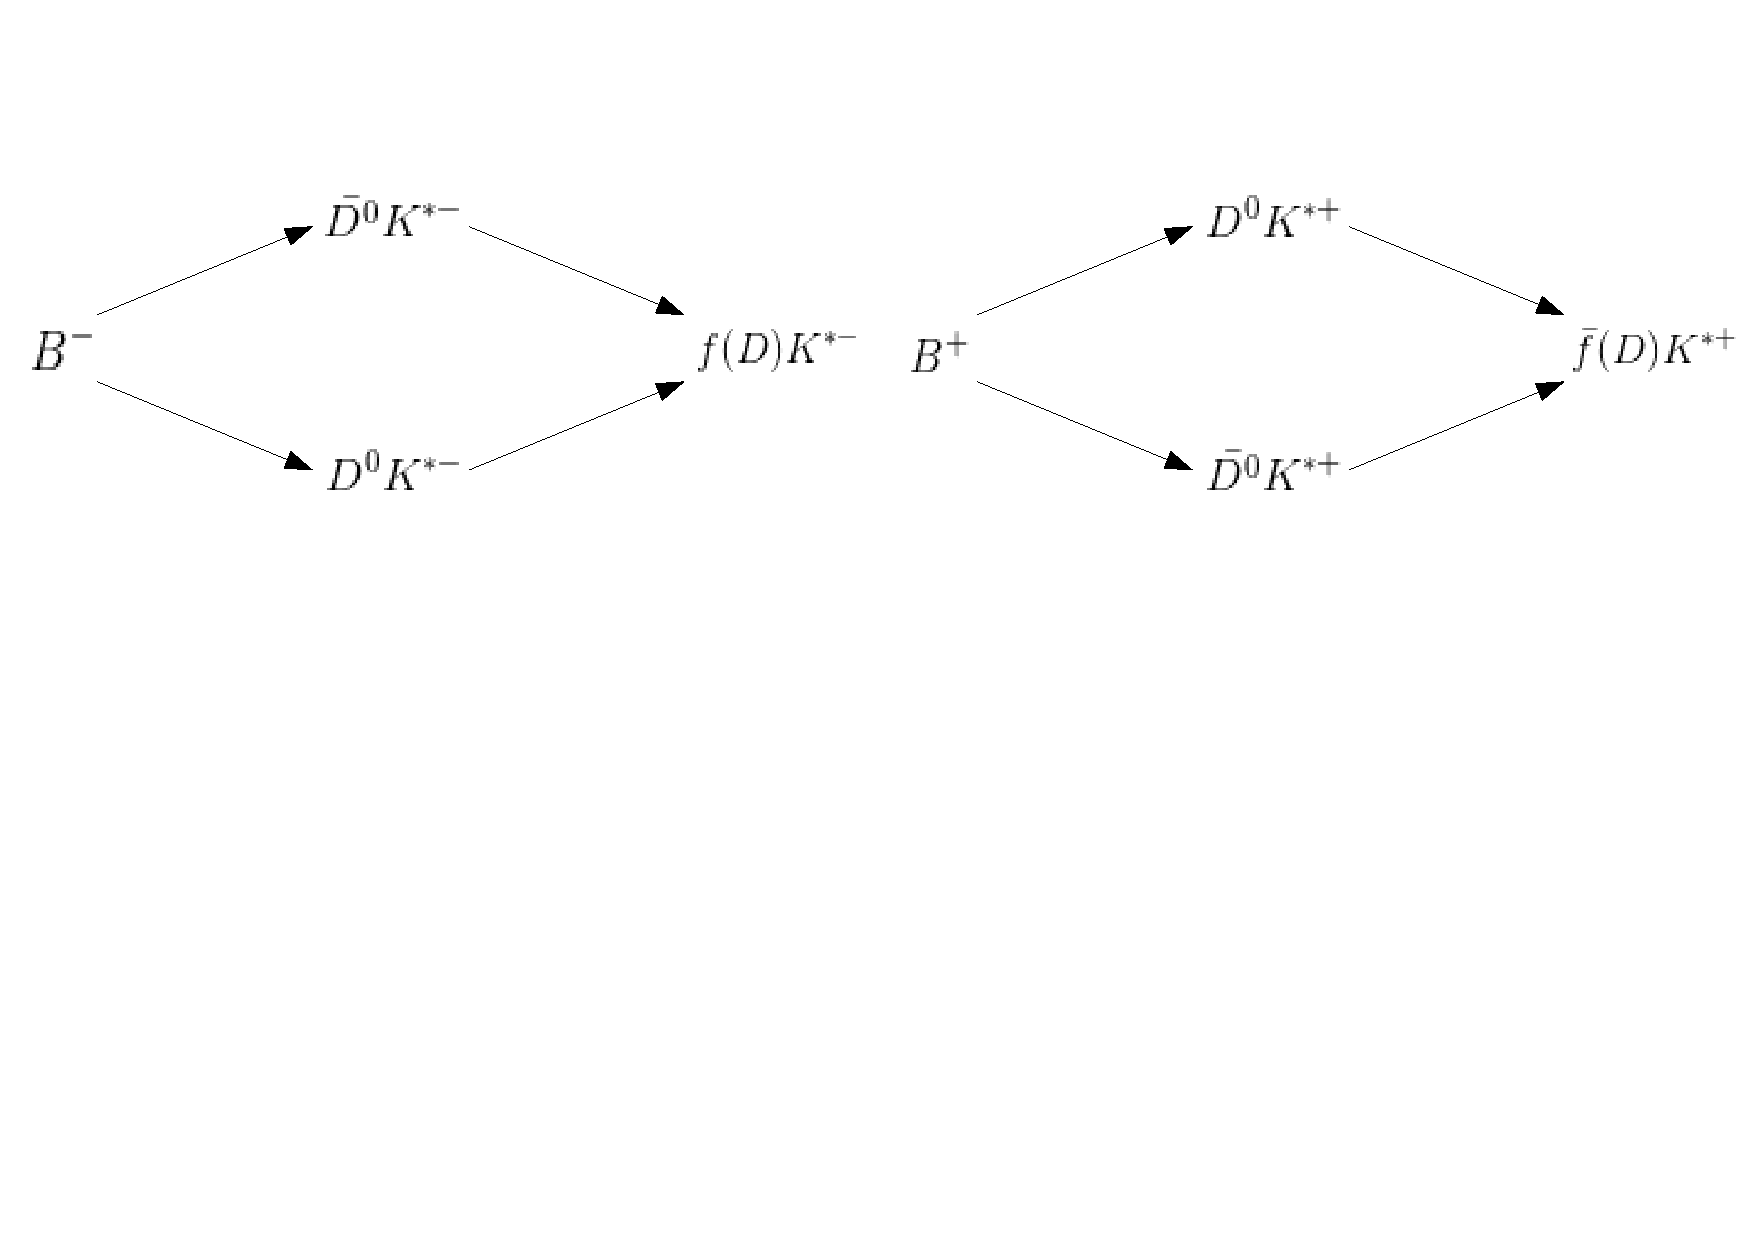
\includegraphics[trim = 0mm 120mm 0mm 30mm,clip,width=\linewidth]{figures/theory/pathDiagrams.pdf}
\put(-420,70) {\tiny $\rb^{DK^*} e^{i(\deltab^{DK^*} - \gamma)}$}
\put(-210,70) {\tiny $\rb^{DK^*} e^{i(\deltab^{DK^*} + \gamma)}$}
\caption{Diagram of the interfering amplitudes of \decay{\Bm}{\D\Kstarm} (left) and \decay{\Bp}{\D\Kstarp} (right)}
\label{paths}
\end{figure}

In the following description we assume \CP violation in the charm sector is negligible, and effects of \D mixing are neglected. The partial widths for the \Bm and \Bp decays are given by \eqn\ref{pwminus} and \ref{pwplus}, where $A_D$ is the amplitude of \decay{\Dz}{f(D)} and $\bar{A_{D}}$ is the amplitude of \decay{\Dzb}{f(D)}.
\begin{align}
\Gamma\left(\decay{\Bm}{[f(D)]\Kstarm}\right) &\propto |A_D|^2 + (\rb^{DK^*})^2 |\bar{A_{D}}|^2 + 2\rb^{DK^*} Re\left[ A_D \bar{A_{D}} e^{-i(\deltab^{DK^*} - \gamma)} \right] \label{pwminus} \\
\Gamma\left(\decay{\Bp}{[f(D)]\Kstarp}\right) &\propto |A_D|^2 + (\rb^{DK^*})^2 |\bar{A_{D}}|^2 + 2\rb^{DK^*} Re\left[ A_D \bar{A_{D}} e^{-i(\deltab^{DK^*} + \gamma)} \right] \label{pwplus}
\end{align}

The values of the complex amplitudes, $A_{D}$ and $\bar{A_{D}}$, depend on the \D meson final state chosen. The sensitivity to \Pgamma can therefore be maximised by judicious choice of \Dz decay mode, through the dependencies of $A_{D}$ and $\bar{A_{D}}$.

\subsection{The GLW method}
\label{sec:theory:glw}

The theorists Gronau, London and Wyler proposed looking at \D decay modes that are \CP eigenstates, referred to as the GLW method~\cite{GL,GW}, such as the \CP-even eigenstates \decay{\D}{\Kp\Km} and \decay{\D}{\pip\pim}. As the final states are \CP-even eigenstates, $A_{D} = \bar{A_{D}}$, the expressions from \eqn\ref{BandDdecaysminus} and \ref{BandDdecaysplus} can be simplified to
\begin{align}
\Gamma\left(\decay{\Bm}{[f_{GLW}]\Kstarm}\right) &\propto 1 + (\rb^{DK^*})^2 + 2\rb^{DK^*}\cos(\deltab^{DK^*} - \gamma) \label{widthBm} \\
\Gamma\left(\decay{\Bp}{[f_{GLW}]\Kstarp}\right) &\propto 1 + (\rb^{DK^*})^2 + 2\rb^{DK^*}\cos(\deltab^{DK^*} + \gamma) \label{widthBp}
\end{align}
assuming that \CP violation in \D decays is negligible and $\mathcal{A}\left(\decay{\Bm}{\Dz\Kstarm}\right) = \mathcal{A}\left(\decay{\Bp}{\Dzb\Kstarp}\right)$. 

The four-body \D decay mode \decay{\D}{\pip\pim\pip\pim} is a self-conjugate decay mode, which can be used to measure \Pgamma via the GLW method provided the fractional \CP-even content is known~\cite{NAYAK20151}. As this mode is not a pure \CP eigenstate, and as such referred to as quasi-GLW mode, its sensitivity to \Pgamma is reduced. The \CP-even fraction, $F_{4\pi}$, measured to be $\sim 0.75$~\cite{charm4pi}, accounts for the dilution effect. The partial widths for this self-conjugate quasi-GLW mode~\cite{NAYAK20151,charm4pi}, corresponding to equations \ref{widthBm} and \ref{widthBp}, are
\begin{align}
\Gamma\left(\decay{\Bm}{[f_{qGLW}]\Kstarm}\right) \propto 1 + (\rb^{DK^*})^2 + 2\rb^{DK^*}\left(2F_{4\pi} - 1\right)\cos(\deltab^{DK^*} - \gamma) \label{widthBm4body} \\
\Gamma\left(\decay{\Bp}{[f_{GLW}]\Kstarp}\right) \propto 1 + (\rb^{DK^*})^2 + 2\rb^{DK^*}\left(2F_{4\pi} - 1\right)\cos(\deltab^{DK^*} + \gamma) \label{widthBp4body}
\end{align}


\subsection{The ADS method}
\label{sec:theory:ads}

The theorists Gronau, London and Wyler proposed looking at \D decay modes where $f(D)$ is a non-\CP eigenstate such as \decay{\D}{\Km\pip}, referred to as the ADS method~\cite{ADS,ADS-2001}. A key feature of this method is that although the \Dz and \Dzb decay to the same final state they proceed by very different amplitudes. The Feynman diagrams for the doubly Cabibbo-favoured \decay{\Dz}{\Km\pip} decay and the doubly Cabibbo-suppressed \decay{\Dz}{\Kp\pim} decay are shown in \fig\ref{fig:D2KPidiagram}.
\begin{figure}[!h]
\centering
\resizebox{0.48\linewidth}{!}{
	\begin{tikzpicture}[scale=0.98]
        % MAP OUT VERTICES (I have 8 of them)
        \coordinate (a) at (0,2); %c quark start
        \coordinate (b) at (0,1); %ubar quark start
        \coordinate (c) at (5,1); %ubar quark end
        \coordinate (d) at (5,2); %s quark end
        \coordinate (e) at (2,2); %start the W+
        \coordinate (f) at (5,2.67); %dbar quark
        \coordinate (g) at (5,3.33); %u quark
        \coordinate (h) at (4.0,3); %W end
        % DRAW LINES
        \draw[antiparticle] (b)  -- (c); %ubar quark
        \draw[particle] (a)  -- (e); %bbar quark
        \draw[particle] (e)  -- (d); %ubar quark 
        \draw[photon] (e) -- (h); %W+
        \draw[antiparticle] (h)  to (g); %W to ubar quark
        \draw[particle] (h)  to (f); %W to s quark 
        %DRAW LABELS
        \node at ($(a)$) [label={[label distance=-4mm] c},left] {};
        \node at ($(b)$) [label={[label distance=-4mm] $\bar{\rm u}$},left] {};
        \node at ($(c)$) [label={[label distance=-4mm] $\bar{\rm u}$},right]{};
        \node at ($(d)$) [label={[label distance=-4mm] s},right] {};
        \node at ($(f)$) [label={[label distance=-4mm] $\bar{\rm d}$},right]{};
        \node at ($(g)$) [label={[label distance=-4mm] u},right]{};
        \node at ($(e)$) [label={[xshift=25pt,yshift=10pt] $W^+$},above] {};

        %ADD BRACES
        \draw
        [black,decorate,decoration={brace,amplitude=5pt},xshift=-20pt,yshift=0pt]
          (0,0.8)  -- (0,2.2) node [black,midway,left=0pt,xshift=-5pt]{\Dz};
        \draw
        [black,decorate,decoration={brace,amplitude=5pt},xshift=20pt,yshift=0pt]
          (5,3.53) -- (5,2.47) node [black,midway,right=0pt,xshift=5pt]{\pip};
         \draw 	[black,decorate,decoration={brace,amplitude=5pt},xshift=20pt,yshift=0pt]
          (5,2.2)  -- (5,0.8) node [black,midway,right=0pt,xshift=5pt] {\Km};
            \end{tikzpicture}
        }
\resizebox{0.47\linewidth}{!}{
\begin{tikzpicture}[scale=0.98]
        % MAP OUT VERTICES (I have 8 of them)
        \coordinate (a) at (0,2); %c quark start
        \coordinate (b) at (0,1); %ubar quark start
        \coordinate (c) at (5,1); %ubar quark end
        \coordinate (d) at (5,2); %d quark end
        \coordinate (e) at (2,2); %start the W+
        \coordinate (f) at (5,2.67); %u quark
        \coordinate (g) at (5,3.33); %sbar quark
        \coordinate (h) at (4.0,3); %W end
        % DRAW LINES
        \draw[antiparticle] (b)  -- (c); %ubar quark
        \draw[particle] (a)  -- (e); %bbar quark
        \draw[particle] (e)  -- (d); %ubar quark 
        \draw[photon] (e) -- (h); %W+
        \draw[antiparticle] (h)  to (g); %W to ubar quark
        \draw[particle] (h)  to (f); %W to s quark 
        %DRAW LABELS
        \node at ($(a)$) [label={[label distance=-4mm] c},left] {};
        \node at ($(b)$) [label={[label distance=-4mm] $\bar{\rm u}$},left] {};
        \node at ($(c)$) [label={[label distance=-4mm] $\bar{\rm u}$},right]{};
        \node at ($(d)$) [label={[label distance=-4mm] d},right]{};
        \node at ($(f)$) [label={[label distance=-4mm] u},right]{};
        \node at ($(g)$) [label={[label distance=-4mm] $\bar{\rm s}$},right]{};
        \node at ($(e)$) [label={[xshift=25pt,yshift=10pt] $W^+$},above] {};

        %ADD BRACES
        \draw
        [black,decorate,decoration={brace,amplitude=5pt},xshift=-20pt,yshift=0pt]
          (0,0.8)  -- (0,2.2) node [black,midway,left=0pt,xshift=-5pt]{\Dz};
        \draw
        [black,decorate,decoration={brace,amplitude=5pt},xshift=20pt,yshift=0pt]
          (5,3.53) -- (5,2.47) node [black,midway,right=0pt,xshift=5pt]{\Kp};
         \draw 	[black,decorate,decoration={brace,amplitude=5pt},xshift=20pt,yshift=0pt]
          (5,2.2)  -- (5,0.8) node [black,midway,right=0pt,xshift=5pt] {\pim};
            \end{tikzpicture}
    }
    \caption{Leading order Feynman diagrams for \decay{\Dz}{\Km\pip} (left) and \decay{\Dz}{\Kp\pim} (right).}
    \label{fig:D2KPidiagram}
\end{figure}

The ratio of the amplitude between \decay{\Dzb}{\Km\pip} and \decay{\Dz}{\Km\pip} is given by\footnote{The \CP operator acting on the state $\ket{\Dz}$ can result in either, $\CP\ket{\Dz} = \ket{\Dzb}$ or $\CP\ket{\Dz} = - \ket{\Dzb}$. This has consequences for the definition of the strong phase difference. In the ADS formalism, which is used here, the definition $\CP\ket{\Dz} = \ket{\Dzb}$ is used resulting in \ref{ratioads}. The alternative definition, $\CP\ket{\Dz} = - \ket{\Dzb}$, used by HFAG and CLEO-c, would result in $r_D^{K\pi}e^{-i(\pi + \delta_D^{K\pi})}$. The consequence of this is, the measured value of the strong phase difference is taken from Refs.~\cite{charmk3pi,LHCb-PAPER-2015-057} must be offset by $180^{\circ}$ when used in this thesis.}
\begin{equation}
\frac{\mathcal{A}\left(\decay{\Dzb}{\Km\pip}\right)}{\mathcal{A}\left(\decay{\Dz}{\Km\pip}\right)} = r_D^{K\pi}e^{-i\delta_D^{K\pi}}
\label{ratioads}
\end{equation}
where, the parameter $r_D^{K\pi}$ is the magnitude of ratio of the amplitudes and $\delta_D^{K\pi}$ is difference in strong phase between the suppressed and favoured decays. These parameters have been previously measured to be $r_D^{K\pi} \sim 0.06$ and $\delta_D^{K\pi} \sim 192^{\circ}$.

This is equivalent to $\bar{A_{D}}/A_{D} = r_D^{K\pi}e^{-i\delta_D^{K\pi}}$ for the case where $f(D)$ is \Km\pip. Similarly, $A_{D}/\bar{A_{D}} = r_D^{K\pi}e^{-i\delta_D^{K\pi}}$ for the case where $f(D)$ is \Kp\pim. Using these expressions, the partial widths from \eqn\ref{BandDdecaysminus} and \ref{BandDdecaysplus} for the various \decay{\Bpm}{\D\Kstarpm} decays with ADS decay modes are given by
\begin{align}
\Gamma\left(\decay{\Bm}{[\Kp\pim]\Kstarm}\right) &\propto (\rb^{DK^*})^2 + (r_D^{K\pi})^2 + 2\rb^{DK^*}r_D^{K\pi}\cos(\deltab^{DK^*} + \delta_D^{K\pi} - \gamma) \label{adsBdecaym} \\
\Gamma\left(\decay{\Bp}{[\Km\pip]\Kstarp}\right) &\propto (\rb^{DK^*})^2 + (r_D^{K\pi})^2 + 2\rb^{DK^*}r_D^{K\pi}\cos(\deltab^{DK^*} + \delta_D^{K\pi} + \gamma) \label{adsBdecayp} \\
\Gamma\left(\decay{\Bm}{[\Km\pip]\Kstarm}\right) &\propto 1 + (\rb^{DK^*})^2(r_D^{K\pi})^2 + 2\rb^{DK^*}r_D^{K\pi}\cos(\deltab^{DK^*} + \delta_D^{K\pi} + \gamma) \label{favBdecaym} \\
\Gamma\left(\decay{\Bp}{[\Kp\pim]\Kstarp}\right) &\propto 1 + (\rb^{DK^*})^2(r_D^{K\pi})^2 + 2\rb^{DK^*}r_D^{K\pi}\cos(\deltab^{DK^*} + \delta_D^{K\pi} - \gamma) \label{favBdecayp} 
\end{align}
In the favoured decay, the pion from the \D meson and that from the \Kstarm meson have opposite charge, while in the suppressed decay the pion from the \D meson and that from the \Kstarm meson have the same charge. The ADS decay mode is a combination of a CKM-favoured \decay{\Bm}{\Dz\Kstarm} decay, followed by a doubly Cabibbo-suppressed \decay{\Dz}{\Kp\pim} decay, and a CKM- and colour-suppressed \decay{\Bm}{\Dzb\Kstarm} decay, followed by a Cabibbo-favoured \decay{\Dzb}{\Kp\pim} decay. Both paths to the same final state have amplitudes of similar size, and interference effects are therefore magnified in comparison to the GLW decay modes, where the decay path via the CKM-favoured \decay{\Bm}{\Dz\Kstarm} dominates.

Two-body \decay{\D}{\Kmp\pipm} decays are characterised by two parameters, an ampiltude ratio and a single strong phase, as illustrated in Eqn~\ref{ratioads}. However for multibody \decay{\D}{\Kmp\pipm\pimp\pipm} decays the strong phase varies over the phase space. Therefore, the amplitude at each point in phasespace must be considered for both the \decay{\D}{\Km\pip\pim\pip} favoured and \decay{\Dz}{\Kp\pim\pip\pim} supressed decays, referred to as $A_{fav}(p)$ and $A_{sup}(p)$. The three hadronic parameters that define the  \decay{\D}{\Km\pip\pim\pip} decay~\cite{charmk3pi,LHCb-PAPER-2015-057} are defined by
\begin{align}
r_D^{K3\pi} &= \frac{\int \mathrm{d}p \left|A_{sup}(p)\right|^2}{\int \mathrm{d}p \left|A_{fav}(p)\right|^2}
\label{rddefinition}
\end{align}
\begin{align}
R_{K3\pi} e^{i\delta_D^{K3\pi}} &= \frac{\int \mathrm{d}p A_{fav}(p)A_{sup}(p)}{\sqrt{\int \mathrm{d}p \left|A_{fav}(p)\right|^2 \int \mathrm{d}p \left|A_{sup}(p)\right|^2}}
\label{Rddefinition}
\end{align}
where $r_D^{K3\pi}$ is the amplitude ratio between suppressed and favoured \decay{\D}{\Km\pip\pim\pip} decays analgous to $r_D^{K\pi}$, $R_{K3\pi}$ is a coherence factor to account for the dilution of the interference effects due to averaging over phasespace, and $\delta_D^{K3\pi}$ is the strong phase difference analagous to $\delta_D^{K\pi}$. These parameters have been previously measured to be $r_D^{K3\pi} \sim 0.0006$, $R_{K3\pi} \sim 0.17$ and $\delta_D^{K3\pi} \sim 28^{\circ}$~\cite{charmk3pi,LHCb-PAPER-2015-057}. Based on the definitions in Eqns~\ref{rddefinition} and \ref{Rddefinition}, the corresponding equations to \eqn\ref{adsBdecaym} - \ref{favBdecayp} are
\begin{align}
\Gamma\left(\decay{\Bm}{[\Kp\pim]\Kstarm}\right) &\propto (\rb^{DK^*})^2 + (r_D^{K3\pi})^2 + 2\rb^{DK^*}R_{K3\pi}r_D^{K3\pi}\cos(\deltab^{DK^*} + \delta_D^{K3\pi} - \gamma) \label{adsBdecaym4body} \\
\Gamma\left(\decay{\Bp}{[\Km\pip]\Kstarp}\right) &\propto (\rb^{DK^*})^2 + (r_D^{K3\pi})^2 + 2\rb^{DK^*}R_{K3\pi}r_D^{K3\pi}\cos(\deltab^{DK^*} + \delta_D^{K3\pi} + \gamma) \label{adsBdecayp4body} \\
\Gamma\left(\decay{\Bm}{[\Km\pip]\Kstarm}\right) &\propto 1 + (\rb^{DK^*})^2(r_D^{K3\pi})^2 + 2\rb^{DK^*}R_{K3\pi}r_D^{K3\pi}\cos(\deltab^{DK^*} + \delta_D^{K3\pi} + \gamma) \label{favBdecaym4body} \\
\Gamma\left(\decay{\Bp}{[\Kp\pim]\Kstarp}\right) &\propto 1 + (\rb^{DK^*})^2(r_D^{K3\pi})^2 + 2\rb^{DK^*}R_{K3\pi}r_D^{K3\pi}\cos(\deltab^{DK^*} + \delta_D^{K3\pi} - \gamma) \label{favBdecayp4body} 
\end{align}
It can be seen from these equations that the four-body coherence factor, $R_{K3\pi}$, modulated the size of the interference term that carries the dependence on \Pgamma.

\subsection{Physical observables}

This thesis aims to measure \Pgamma as well as hadronic parameters of \btodkst decays using the methods and equations discussed in Sections \ref{sec:theory:glw} and \ref{sec:theory:ads}. However, experimental considerations must be taken into account when developing the strategy to measure these parameters. For example, the use of the parameters $\rb^{DK^*}$ and $\deltab^{DK^*}$ in Section \ref{sec:theory:gamma}, assumes that a pure sample of \btodkst decays is available. Section \ref{sec:theory:kappa} introduces the coherence factor, $\kappa$, which deals with the contamination from other \decay{\Bm}{\D\KS\pim} processes in order to extract the parameters of interest. Section \ref{sec:theory:observables} describes the experimental quantities that are measured in this analysis in order to gain maximum senstivity to \Pgamma. 

\subsubsection{Coherence factor}
\label{sec:theory:kappa}

As discussed in this chapter, this thesis considers \decay{\Bm}{\D\Kstarm}, \decay{\Kstarm}{\KS\pim} decays. As the \Kstarm meson has a large natural width (about 50 MeV~\cite{PDG2016}), non-resonant \decay{\Bm}{\D\KS\pim} processes may be non-negligible in this region. Equations \ref{pwminus} and \ref{pwplus} assume that it is possible to gain a sample of pure \decay{\Bm}{\D\Kstarm}, \decay{\Kstarm}{\KS\pim} decays, with no other contributions from other \decay{\Bm}{\D\KS\pim} decays. However, experimentally it is not possible to completely separate the \decay{\Bm}{\D\Kstarm} decays. Therefore, it is necessary to consider the effect of other resonant and non-resonant \decay{\Bm}{\D\KS\pim} decays on the experimental measurements of the physics parameters, $\rb^{DK^*}$, $\rb^{DK^*}$ and \Pgamma. The amplitudes and phases of the different decays would be different at each point in \decay{\Bm}{\D\KS\pim} phasespace, as given by
\begin{align*}
A(B^- \to D^0 X^-) &= A_c(p) e^{i\delta_c(p)} \\
A(B^- \to \bar{D^0} X^-) &= A_u(p) e^{i(\delta_u(p) - \gamma)}
\end{align*}
where p is the $\left(m^2(\KS\pim),m^2(\D\pim)\right)$ coordinate in the \decay{\Bm}{\D\KS\pim} Dalitz plot, $A_u(p)$ and $A_c(p)$ are the moduli of the \decay{\bquark}{\uquark} and \decay{\bquark}{\cquark} amplitudes, and $\delta_{c,u}(p)$ represent the strong phases of the relevant decay amplitudes. The symbol $X^-$ represents a resonant or non-resonant \KS\pim pair, which could be produced by the decay of the \Kstarm meson or by other contributions to the \decay{\Bm}{\D\KS\pim} final state. The amplitudes of the \Bp decays can be expressed as 
\begin{align*}
A(\decay{\Bp}{\Dzb X^+}) &= A_c(p) e^{i\delta_c(p)} \\
A(\decay{\Bp}{\Dz X^+}) &= A_u(p) e^{i(\delta_u(p) + \gamma)}
\end{align*}
Due to the large natural width of the \Kstarm, in the region near the \Kstarm mass interference may occur between the signal \Kstarm decay amplitude and amplitudes due to other \decay{\Bm}{\D\KS\pim} contributions, for example higher \KS\pim resonances and non-resonant decays. The interfering contributions dilute the sensitivity to \Pgamma, which is quantified by a coherence factor, $\kappa$, where $0 \leq \kappa \leq 1$ and $\kappa = 1$ denotes a pure $K^{*-}$ contribution, giving maximum sensitivity to \Pgamma. The parameters \rb, \deltab and $\kappa$ for \btodkst decays are defined as
\begin{align}
r_B &= \frac{\Gamma(B^- \to \bar{D^0}X^-)}{\Gamma(B^- \to D^0X^-)} = \frac{\int \left|A_u(p)\right|^2 \mathrm{d}p}{\int \left|A_c(p)\right|^2 \mathrm{d}p}
\label{rbdefinition}
\end{align}
\begin{align}
\kappa e^{i\delta_B} &= \frac{\int \mathrm{d}p A_c(p)A_u(p)e^{i\delta(p)}}{\sqrt{\int \mathrm{d}p \left|A_u(p)\right|^2 \int \mathrm{d}p \left|A_c(p)\right|^2}}
\label{kappadefinition}
\end{align}
where p represents a point in phasespace, $0 \leq \delta_B \leq 2\pi$ and the integration is performed over a defined \Kstarm region. The amplitudes include both resonant $B^- \to DK^{*-}$ and non-resonant \decay{\Bm}{\D\KS\pim} contributions, which is what the coherence factor, $\kappa$, accounts for. The parameters \rb, \deltab and $\kappa$ depend on the region of \decay{\Bm}{\D\KS\pim} phasespace that is integrated over in Equations \ref{rbdefinition} and \ref{kappadefinition}. In order to maximise sensitivity to \Pgamma an integration region should be chosen that produces the largest value of $\kappa$.

In the following description we assume \CP violation in the charm sector is negligible, and effects of \D mixing are neglected. The partial widths for the \Bm and \Bp decays are given by \eqn\ref{partialwidthminus} and \ref{partialwidthplus}, where $A_D$ is the amplitude of \decay{\Dz}{f(D)} and $\bar{A_{D}}$ is the amplitude of \decay{\Dzb}{f(D)}.
\begin{align}
\frac{d\Gamma\left(\decay{\Bm}{[f(D)]X^-}\right)}{dp} &\propto | A_c(p) e^{i\delta_c(p)}A_{D} + A_u(p) e^{i(\delta_u(p) - \gamma)}\bar{A_{D}} |^2 \label{partialwidthminus} \\
\frac{d\Gamma\left(\decay{\Bp}{[f(D)]X^-}\right)}{dp} &\propto | A_u(p) e^{i(\delta_u(p) + \gamma)}\bar{A_{D}} + A_c(p) e^{i\delta_c(p)}A_{D} |^2 \label{partialwidthplus}
\end{align}

Expanding and integrating over the defined \Kstar region gives,
\begin{align}
\Gamma\left(\decay{\Bm}{[f(D)]X^-}\right) &\propto |A_D|^2 + \rb^2 |\bar{A_{D}}|^2 + 2\kappa\rb Re\left[ A_D \bar{A_{D}} e^{-i(\deltab - \gamma)} \right] \label{BandDdecaysminus} \\
\Gamma\left(\decay{\Bp}{[f(D)]X^-}\right) &\propto |A_D|^2 + \rb^2 |\bar{A_{D}}|^2 + 2\kappa\rb Re\left[ A_D \bar{A_{D}} e^{-i(\deltab + \gamma)} \right] \label{BandDdecaysplus}
\end{align}

\subsubsection{\CP observables}
\label{sec:theory:observables}

Using the GLW and ADS methods, discussed in Sections \ref{sec:theory:glw} and \ref{sec:theory:ads}, observable quantities are constructed that can be used to extract \rb, \deltab and \Pgamma. This is achieved by considering asymmetries between the decay rates \Bm and \Bp decays, as well as ratios of decay rates in comparison to the favoured modes for the different \Dz final states. No \CP asymmetry is expected in the two- and four-body favoured \Dz decay modes. Twelve quantities, collectively referred to as \CP observables, are measured in this analysis:

\begin{itemize}
\item{The \CP asymmetry for the favoured decay mode
\begin{equation}
A_{\kaon\pi} = \frac{\Gamma\left(\decay{\Bm}{\D(\Km\pip)\Kstarm}\right) - \Gamma\left(\decay{\Bp}{\D(\Kp\pim)\Kstarp}\right)}{\Gamma\left(\decay{\Bm}{\D(\Km\pip)\Kstarm}\right) + \Gamma\left(\decay{\Bp}{\D(\Kp\pim)\Kstarp}\right)} \text{ .}
\label{eqn:Akpi}
\end{equation}}
\item{The \CP asymmetry for the \decay{\D}{\Kp\Km} decay mode
\begin{equation}
A_{\kaon\kaon} = \frac{\Gamma\left(\decay{\Bm}{\D(\Kp\Km)\Kstarm}\right) - \Gamma\left(\decay{\Bp}{\D(\Kp\Km)\Kstarp}\right)}{\Gamma\left(\decay{\Bm}{\D(\Kp\Km)\Kstarm}\right) + \Gamma\left(\decay{\Bp}{\D(\Kp\Km)\Kstarp}\right)} \text{ . }
\label{eqn:Akk}
\end{equation}
}
\item{The \CP asymmetry for the \decay{\D}{\pip\pim} decay mode
\begin{equation}
A_{\pi\pi} = \frac{\Gamma\left(\decay{\Bm}{\D(\pip\pim)\Kstarm}\right) - \Gamma\left(\decay{\Bp}{\D(\pip\pim)\Kstarp}\right)}{\Gamma\left(\decay{\Bm}{\D(\pip\pim)\Kstarm}\right) + \Gamma\left(\decay{\Bp}{\D(\pip\pim)\Kstarp}\right)} \text{ . }
\label{eqn:Apipi}
\end{equation}}
\item{The ratio of the rate for the \decay{\D}{\Kp\Km} decay mode to that of the favoured decay mode, scaled by the branching fractions
\begin{multline}
R_{\kaon\kaon} = \frac{\Gamma\left(\decay{\Bm}{\D(\Kp\Km)\Kstarm}\right) + \Gamma\left(\decay{\Bp}{\D(\Kp\Km)\Kstarp}\right)}{\Gamma\left(\decay{\Bm}{\D(\Km\pip)\Kstarm}\right) + \Gamma\left(\decay{\Bp}{\D(\Kp\pim)\Kstarp}\right)} \\ \times \frac{\BR(D^0 \to K^-\pi^+)}{\BR(D^0 \to K^+K^-)} \text{ . }
\label{eqn:Rkk}
\end{multline}
}
\item{The ratio of the rate for the \decay{\D}{\pip\pim} decay mode to that of the favoured decay mode, scaled by the branching fractions
\begin{multline}
R_{\pi\pi} = \frac{\Gamma\left(\decay{\Bm}{\D(\pip\pim)\Kstarm}\right) + \Gamma\left(\decay{\Bp}{\D(\pip\pim)\Kstarp}\right)}{\Gamma\left(\decay{\Bm}{\D(\Km\pip)\Kstarm}\right) + \Gamma\left(\decay{\Bp}{\D(\Kp\pim)\Kstarp}\right)} \\ \times \frac{\BR(D^0 \to K^-\pi^+)}{\BR(D^0 \to \pi^+\pi^-)} \text{ . }
\label{eqn:Rpipi}
\end{multline}}
\item{The ratio of the rate for the ADS decay mode to that of the favoured decay mode for \Bp decays
\begin{equation}
R^+_{K\pi} = \frac{\Gamma\left(\decay{\Bp}{\D(\Km\pip)\Kstarp}\right)}{\Gamma\left(\decay{\Bp}{\D(\Kp\pim)\Kstarp}\right)} \text{ . }
\label{eqn:Rplus}
\end{equation}
}
\item{The ratio of the rate for the ADS decay mode to that of the favoured decay mode for \Bm decays
\begin{equation}
R^-_{K\pi} = \frac{\Gamma\left(\decay{\Bm}{\D(\Kp\pim)\Kstarm}\right)}{\Gamma\left(\decay{\Bm}{\D(\Km\pip)\Kstarm}\right)} \text{ . }
\label{eqn:Rminus}
\end{equation}
}
\item{The \CP asymmetry for the favoured \decay{\Dz}{\Km\pip\pim\pip} decay mode
{\footnotesize
\begin{equation}
A_{\kaon\pi\pi\pi} = \frac{\Gamma\left(\decay{\Bm}{\D(\Km\pip\pim\pip)\Kstarm}\right) - \Gamma\left(\decay{\Bp}{\D(\Kp\pim\pip\pim)\Kstarp}\right)}{\Gamma\left(\decay{\Bm}{\D(\Km\pip\pim\pip)\Kstarm}\right) + \Gamma\left(\decay{\Bp}{\D(\Kp\pim\pip\pim)\Kstarp}\right)} \text{ . }
\label{eqn:Akpipipi}
\end{equation}}}
\item{The \CP asymmetry for the \decay{\D}{\pip\pim\pip\pim} decay mode
{\footnotesize
\begin{equation}
A_{\pi\pi\pi\pi} = \frac{\Gamma\left(\decay{\Bm}{\D(\pip\pim\pip\pim)\Kstarm}\right) - \Gamma\left(\decay{\Bp}{\D(\pip\pim\pip\pim)\Kstarp}\right)}{\Gamma\left(\decay{\Bm}{\D(\pip\pim\pip\pim)\Kstarm}\right) + \Gamma\left(\decay{\Bp}{\D(\pip\pim\pip\pim)\Kstarp}\right)} \text{ . }
\label{eqn:Apipipipi}
\end{equation}
}}
\item{The ratio of the rate for the \decay{\D}{\pip\pim\pip\pim} decay mode to that of the favoured decay mode, scaled by the branching fractions
{\footnotesize
\begin{multline}
R_{\pi\pi\pi\pi} = \frac{\Gamma\left(\decay{\Bm}{\D(\pip\pim\pip\pim)\Kstarm}\right) + \Gamma\left(\decay{\Bp}{\D(\pip\pim\pip\pim)\Kstarp}\right)}{\Gamma\left(\decay{\Bm}{\D(\Km\pip\pim\pip)\Kstarm}\right) + \Gamma\left(\decay{\Bp}{\D(\Kp\pim\pip\pim)\Kstarp}\right)} \\
\times \frac{\mathcal{B}(D^0 \to \Km\pip\pim\pip)}{\mathcal{B}(D^0 \to \pip\pim\pip\pim)} \text{ . }
\label{eqn:Rpipipipi}
\end{multline}}}
\item{The ratio of the rate for the four-body ADS decay mode to that of the four-body favoured decay mode for \Bp decays
\begin{equation}
R^+_{K\pi\pi\pi} = \frac{\Gamma\left(\decay{\Bp}{\D(\Km\pip\pim\pip)\Kstarp}\right)}{\Gamma\left(\decay{\Bp}{\D(\Kp\pim\pip\pim)\Kstarp}\right)} \text{ . }
\label{eqn:Rplus4body}
\end{equation}
}
\item{The ratio of the rate of the four-body ADS decay mode to that of the four-body favoured decay mode for \Bm decays
\begin{equation}
R^-_{K\pi\pi\pi} = \frac{\Gamma\left(\decay{\Bm}{\D(\Kp\pim\pip\pim)\Kstarm}\right)}{\Gamma\left(\decay{\Bm}{\D(\Km\pip\pim\pip)\Kstarm}\right)} \text{ . }
\label{eqn:Rminus4body}
\end{equation}
}
\end{itemize}

\noindent
The asymmetries $A_{\kaon\pi}$ and $A_{\kaon\pi\pi\pi}$ should be essentially zero due to the very small interference expected in the configuration of \B and \D decays. Due to negligible direct \CP violation in \D decays~\cite{charmcpv}, the observables $A_{\kaon\kaon}$ and $A_{\pi\pi}$ should be equal and are often labelled together as $A_{\CP+}$; similarly the observables $R_{\kaon\kaon}$ and $R_{\pi\pi}$ should be equal and are labelled $R_{\CP+}$. \footnote{The analogous observables to $R_{\CP+}$ and $A_{\CP+}$ for the ADS mode are $R_{ADS}$ and $A_{ADS}$. However, $R_{ADS}$ and $A_{ADS}$ are not used for the ADS decay mode, instead the ratios are measured separately for the positive and negative charges. The reason for this choice is that the uncertainty in $A_{ADS}$ depends on the value of $R_{ADS}$, therefore these observables are statistically dependent, raising problems for the low yields expected in the ADS mode. Hence the statistically independent observables $R^+_{K\pi}$ and $R^-_{K\pi}$ are preferred.}

The \CP observables measured in this analysis can be related to the physics parameters to be determined, namely \Pgamma, $r_B$ and $\delta_B$. Given there is a negligible effect from both charm mixing~\cite{charmmixing} and \CP violation in \D decays~\cite{charmcpv}, the relationships between the \CP observables and physics parameters are given in the following equations,

\begin{equation}
A_{\CP+} = \frac{2 \kappa r_B\sin\delta_B\sin\gamma}{1 + r_B^2 + 2 \kappa r_B\cos\delta_B\cos\gamma} \text{ ,}
\label{exp_Acp}
\end{equation}
\begin{equation}
R_{\CP+} = 1 + r_B^2 + 2 \kappa r_B\cos\delta_B\cos\gamma \text{ ,}
\label{exp_Rcp}
\end{equation}
\begin{equation}
R^{\pm}_{K\pi} = \frac{r_B^2 + \left(r_D^{K\pi}\right)^2 + 2\kappa r_B r_D^{K\pi} \cos(\delta_B + \delta_D^{K\pi} \pm \gamma)}{1 + r_B^2\left(r_D^{K\pi}\right)^2 + 2\kappa r_B r_D^{K\pi} \cos(\delta_B - \delta_D^{K\pi} \pm \gamma)} \text{ ,}
\label{exp_Rpm}
\end{equation}
\begin{equation}
A_{\pi\pi\pi\pi} = \frac{2 \kappa\left(2F_{4\pi} - 1\right) r_B\sin\delta_B\sin\gamma}{1 + r_B^2 + 2 \kappa\left(2F_{4\pi} - 1\right) r_B\cos\delta_B\cos\gamma} \text{ ,}
\label{exp_A4pi}
\end{equation}
\begin{equation}
R_{\pi\pi\pi\pi} = 1 + r_B^2 + 2 \kappa\left(2F_{4\pi} - 1\right) r_B\cos\delta_B\cos\gamma \text{ ,}
\label{exp_R4pi}
\end{equation}
\begin{equation}
R^{\pm}_{K\pi\pi\pi} = \frac{r_B^2 + \left(r_D^{K3\pi}\right)^2 + 2\kappa r_B \kappa_{K3\pi} r_D^{K3\pi} \cos(\delta_B + \delta_D^{K3\pi} \pm \gamma)}{1 + \left(r_Br_D^{K3\pi}\right)^2 + 2\kappa r_B \kappa_{K3\pi} r_D^{K3\pi} \cos(\delta_B - \delta_D^{K3\pi} \pm \gamma)} \text{ .}
\label{exp_Rpm4body}
\end{equation}

These six relationships contain 10 unknown parameters: the three parameters of interest, namely \rb, \deltab and \Pgamma, the coherence factor, $\kappa$, relating to the \Bm decay, which has a value specific to this analysis and six parameters describing the various \Dz decays, namely $r_D^{K\pi}$, $\delta_D^{K\pi}$, $r_D^{K3\pi}$, $\delta_D^{K3\pi}$, $R_{K3\pi}$ and $F_{4\pi}$, which have all been previously measured~\cite{charm4pi,charmk3pi,LHCb-PAPER-2015-057}. Therefore, the strategy taken in this thesis to extract \rb, \deltab and \Pgamma is to take the six parameters describing the various \Dz decays directly from existing measurements.


\section{Previous \Pgamma measurements with \decay{\Bpm}{\D K^{(*)\pm}} decays}

The \decay{\Bm}{\D\Km} channel is a very important mode for tree level \Pgamma measurements, as it is straightforward to reconstruct and has a fairly high branching fraction of $3.7 \times 10^{-4}$~\cite{PDG2016}. This \decay{\Bm}{\D\Km} channel is thoroughly exploited at \lhcb having yielded many \Pgamma sensitive measurements using an extensive range of \D meson final states:
\begin{itemize}
\item \decay{\D}{\Kp\pim}, \Kp\Km, \pip\pim~\cite{LHCb-PAPER-2017-021},
\item \decay{\D}{\Kp\pim\pip\pim}, \pip\pim\pip\pim~\cite{LHCb-PAPER-2016-003},
\item \decay{\D}{\Kp\pim\piz}, \Kp\Km\piz, \pip\pim\piz~\cite{LHCb-PAPER-2015-014},
\item \decay{\D}{\KS\Kp\Km}, \KS\pip\pim~\cite{LHCb-PAPER-2014-041},
\item \decay{\D}{\KS\Kp\Km}~\cite{LHCb-PAPER-2013-068}.
\end{itemize}

Other experiments, other \Pgamma sensitive decays \Bz and \Bs. Why is \Pgamma less well known despite it being the only tree level angle?

The \decay{\Bm}{\D\Kstarm} channel is analogous to the \decay{\Bm}{\D\Km} in its physical properties as well as having a comparable branching fraction of $5.3 \times 10^{-4}$~\cite{PDG2016}. However, prior to the work presented in this thesis the \decay{\Bm}{\D\Kstarm} channel had not been investigated at \lhcb. The \Kstarm decays almost exclusively to \Kz\pim and \Km\piz final states, both of which involve a neutral particle; this makes \decay{\Bm}{\D\Kstarm} much more difficult to reconstruct at \lhcb than \decay{\Bm}{\D\Km}. 

The \decay{\Bm}{\D\Kstarm} channel has previously been investigated by the BaBar collaboration using a variety of \CP-even, \CP-odd and non-\CP two-body \D decay modes, namely \Km\Kp, \pim\pip, \KS\piz, $\KS\phi$, $\KS\omega$ and \Km\pip~\cite{BaBarDKstar}. This study produced confidence levels for \Pgamma, excluding $[85,99]^{\circ}$ at the level of two sigma. Also, both the BaBar and Belle collaborations have performed studies on \decay{\Bm}{\D\Kstarm} with \decay{\D}{\KS\pip\pim}~\cite{BaBarGGSZ,BelleGGSZ}, obtaining results of $\Pgamma = (76 \pm 22 \pm 5 \pm 5)^{\circ}$ (mod $180^{\circ}$) and $\Pgamma = (53^{+15}_{-18} \pm 3 \pm 9)^{\circ}$, respectively. In all of these measurements the \Kstarm meson is reconstructed in the \KS\pim mode, with \decay{\KS}{\pip\pim}.

In this analysis, the \decay{\Bm}{\D\Kstarm} channel is investigated, with \decay{\Kstarm}{\KS\pim} and \decay{\KS}{\pim\pip}, where the \Dz meson in reconstructed in its decay to two or four charged kaons and/or pions. The \Kstarm meson can be reconstructed from its decay to \Km\piz, however, the \piz meson decays almost exclusively to two photons, which are difficult to reconstruct, and therefore the \piz meson has a much poorer reconstruction efficiency than the \KS meson. Also, due to the properties of the detector, the reconstruction efficiency of the \piz has a larger uncertainty. Both the reduced statistics due to the poor reconstruction efficiency and the large uncertainty of the reconstruction efficiency, it is not considered beneficial to include the reconstruction of the \Kstarm meson in the \Km\piz mode.

\section{Analysis overview}

The work presented measures the \CP observables in \decay{\Bm}{\D\Kstarm} decays as well as considering the interpretation of these observables in terms of \rb, \deltab and \Pgamma. The analysis strategy is to first develop a procedure, based on our understanding of the data, to select \decay{\Bm}{\D(\Km\pip)\Kstarm} signal decays while removing unwanted background events, discussed in Section \ref{sec:selection}. The same selection with a few adjustments can subsequently be applied to the other two- and four- body \D decay modes. After applying this selection, a fit model is developed to described the \B mass distribution of the remaining \decay{\Bm}{\D(\Km\pip)\Kstarm} candidates, detailed in Section \ref{sec:massfit}. This model must include various components in order to fully describe the shape of the \B mass distribution. Using the fit model developed based on the \decay{\Bm}{\D(\Km\pip)\Kstarm} mode, a simultaneous fit is then performed to all the seven \D modes separated by \B charge in order to extract the \CP observables defined in \eqn\ref{eqn:Akpi}-\ref{eqn:Rminus4body}, detailed in Section \ref{ch:5-cpfit}. Section \ref{ch:6-interpretation} discusses determination of $\kappa$ using \eqn\ref{kappadefinition} as well as the interpretation of the \CP observables using \eqn\ref{exp_Acp}-\ref{exp_Rpm4body}, in terms of the physics parameters: \rb, \deltab and \Pgamma.